\chapter{Trasmissione con UART}

\section*{Obiettivo}
Trasmettere un array di numeri utilizzando la seriale e leggere questi numeri utilizzando MATLAB.

\section*{Svolgimento\footnote{\href{https://github.com/fdila/electronics-experimentation/tree/main/Exp04}{Il codice è disponibile nella repository, cartella Exp04}}}

Tramite CubeMX andiamo ad impostare la periferica USART3 per trasmettere e ricevere dati, impostiamo il baudrate a 9600 e abilitiamo l'interrupt associato.

Nella fase di setup abilitiamo la seriale e abilitiamo anche l'interrupt associato alla ricezione di un byte.
\begin{minted}
[
frame=lines,
framesep=2mm,
baselinestretch=1.2,
fontsize=\footnotesize,
]{C}
//enable USART
USART3->CR1 |= USART_CR1_UE;
//enable RX interrupt
USART3->CR1 |= USART_CR1_RXNEIE;
\end{minted}

Quando riceveremo un byte sulla seriale verrà chiamata la routine di interrupt associata a USART3.
Controlliamo cosa ha sollevato l'interrupt andando a guardare il registro SR.
Se siamo entrati nell'interrupt perchè è stato ricevuto un byte andiamo a controllare cosa abbiamo ricevuto.
Se abbiamo ricevuto un 10 significa, per nostra convenzione, che MATLAB ha richiesto i dati. 

Andiamo quindi ad abilitare l'interrupt TXE, che viene sollevato ogni volta che il registro DR è vuoto.
Ogni volta che viene sollevato questo interrupt, se abbiamo ancora dati da trasmettere, andiamo a chiamare la funzione tx\_fun(), che restituisce il byte che dobbiamo inviare.
Mettiamo questo byte nel registro DR: la scrittura nel registro DR fa quindi partire automaticamente la trasmissione.

\begin{minted}
[
frame=lines,
framesep=2mm,
baselinestretch=1.2,
fontsize=\footnotesize,
]{C}
void USART3_IRQHandler(void)
{
  /* USER CODE BEGIN USART3_IRQn 0 */
	
	if (USART3->SR & USART_SR_TXE){
		if(tx_index < tx_length){
			USART3->DR = tx_fun();
		} else {
			tx_index = 0;
			USART3->CR1 &= ~USART_CR1_TXEIE;
		}
	}
	
	if (USART3->SR & USART_SR_RXNE){
		uint8_t comando;
		comando = USART3->DR;
		if(comando == 10) {
			USART3->CR1 |= USART_CR1_TXEIE;
		}
	}
	
	
  /* USER CODE END USART3_IRQn 0 */
  HAL_UART_IRQHandler(&huart3);
  /* USER CODE BEGIN USART3_IRQn 1 */

  /* USER CODE END USART3_IRQn 1 */
}
\end{minted}

Abbiamo 3 variabili globali per permettere la trasmissione: un buffer, l'indice a cui ci troviamo nel buffer e la lunghezza in byte del buffer.
Il buffer contiene interi senza segno a 16 bit, ma noi dobbiamo accedere ai singoli byte per poterli inviare sulla seriale.

Andiamo quindi a creare un puntatore a 8 bit all'indirizzo del buffer, e usiamo questo puntatore per accedere ai byte. Ogni volta che viene chiamata la funzione andiamo a prendere dalla memoria un byte e aumentiamo l'indice. L'indice ci dice a che punto siamo nel buffer inteso come numero di byte.

\begin{minted}
[
frame=lines,
framesep=2mm,
baselinestretch=1.2,
fontsize=\footnotesize,
]{C}
uint16_t tx_buffer[] = {10, 20, 30, 40, 50, 60, 70, 80, 90, 100};
uint8_t tx_index = 0;
uint8_t tx_length = sizeof(tx_buffer);

uint8_t tx_fun(void){
	uint8_t* pointer = (uint8_t*) tx_buffer;
	uint8_t to_tx = *(pointer + tx_index);
	
	if (tx_index < tx_length)
		tx_index++;
	return to_tx;
}
\end{minted}

Da MATLAB apriamo lo strumento \textit{Instrument Control}: da qui possiamo aprire la connessione con la seriale, inviare il byte '10' e ricevere i dati inviati dal microcontrollore.

Possiamo poi andare a vedere con l'oscilloscopio la forma di onda generata dalla seriale.

Possiamo vedere quest'onda sia come segnale "digitale", ovvero vedendo i valori sotto a una certa soglia come 0, e i valori sopra una certa soglia come 1, sia come segnale "analogico" andando a vedere la tensione.

Dal punto di vista digitale possiamo andare a vedere come è fatta la trasmissione di un byte con la seriale:
di base, quando non si sta trasmettendo/ricevendo il segnale è alto, abbiamo poi un bit di "start" basso, gli 8 bit trasmessi e un bit di stop.

\begin{figure}[htb]
\centering
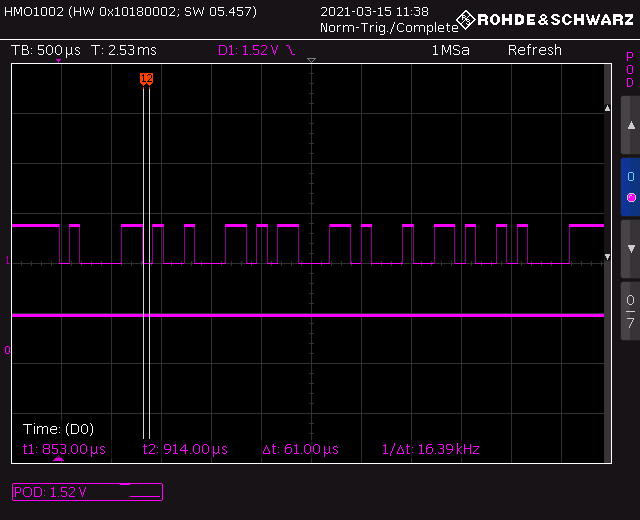
\includegraphics[width=\textwidth]{assets/exp3/SCR02.PNG}
\caption{Vista "digitale"}
\end{figure}

Dal punto di vista analogico notiamo che la tensione del segnale non genera un'onda quadra perfetta ma abbiamo comunque un certo tempo in cui il segnale passa da basso ad alto (e  viceversa).
\begin{figure}[htb]
\centering
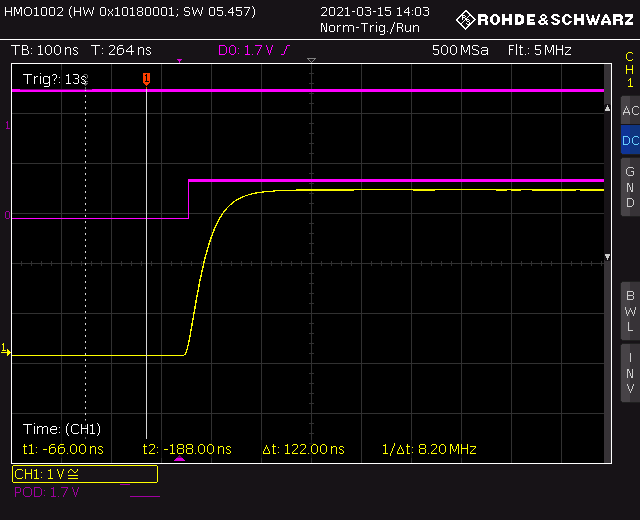
\includegraphics[width=\textwidth]{assets/exp3/SCR07.PNG}
\caption{Vista "analogica"}
\end{figure}